\chapter{Funkcija}


\section{Funkcija}

    \subsection*{Preslikava}

        Naj bosta $\mathcal{X}$ in $\mathcal{Y}$ neprazni množici. \\
        \textbf{Preslikava} $f$ sestoji iz:
        \begin{itemize}
            \item množice $\mathcal{X}$, ki ji pravimo \textbf{domena},
            \item množice $\mathcal{Y}$, ki ji pravimo \textbf{kodomena} in 
            \item \textbf{prirejanja}, ki vsakemu elementu $x$ domene priredi natanko en element $y$ kodomene.
        \end{itemize}

        $$\begin{aligned}
            f&: \mathcal{X}\to\mathcal{Y} \\ f&: x\mapsto y
        \end{aligned}  $$
    

        Elemente $x$ kodomene $\mathcal{X}$ imenujemo \textbf{originali} preslikave.
        \\ Če elementu $x$ priredimo element $y$ iz kodomene, potem imenujemo $y$ \textbf{slika} elemeta $x$.

        Preslikavo lahko podamo s predpisom, puščičnim diagramom, besednim opisom ...





    \subsection*{Funkcija}

        Naj bosta $\mathcal{X}$ in $\mathcal{Y}$ neprazni številski množici. \\
        \textbf{Funkcija} $f$ je preslikava med številskima množicama $\mathcal{X}$ in $\mathcal{Y}$:
        $$f: \mathcal{X}\to\mathcal{Y}.$$


        Število $y$ je \textbf{funkcijska vrednost} števila $x$, če se število $x$ preslika v število $y$. 
        $$ f(x)=y $$

        $x$ je neodvisna spremenjlivka, $f(x)$ je od $x$ odvisna spremenljivka.



        V nekaterih primerih za opis funkcije uporabimo poseben izraz:
        \begin{itemize}
            \item $f:\mathcal{X}\to\mathbb{R}; \mathcal{X}\subseteq\mathbb{R}$ -- realna funkcija realne spremenljivke;
            \item $f:\mathcal{X}\to\mathbb{R}; \mathcal{X}\subseteq\mathbb{N}$ -- realna funkcija naravne spremenljivke;
            \item $f:\mathcal{X}\to\mathbb{N}; \mathcal{X}\subseteq\mathbb{R}$ -- naravna funkcija realne spremenljivke;
            \item $f:\mathcal{X}\to\mathbb{N}; \mathcal{X}\subseteq\mathbb{N}$ -- naravna funkcija naravne spremenljivke.
        \end{itemize}



    \subsection*{Definicijsko območje in zaloga vrednosti}

    \subsubsection*{Definicijsko območje}
        \textbf{Definicijsko območje} preslikave ali funkcije $f:\mathcal{X}\to\mathcal{Y}$ je množica vseh originalov, ki jih v danem primeru opazujemo. 
        Oznaka: $D_f$.                

        Za definicijsko območje navadno vzamemo največjo možno množico, za katero je predpis funkcije veljaven/definiran.

        
    \subsubsection*{Zaloga vrednosti}
        \textbf{Zaloga vrednosti} preslikave ali funkcije $f:\mathcal{X}\to\mathcal{Y}$ je množica vseh slik oziroma funkcijskih vrednosti.
        Oznaka: $Z_f$.

        Zaloga vrednosti $Z_f$ je podmnožica kodomene $\mathcal{Y}$: $Z_f\subseteq \mathcal{Y}$.





%%%% naloge

    \begin{naloga}
        Funkcijo $f: A\to B$ predstavite s tabelo. Izračunajte, kam posamezna funkcija preslika $x=1$.
        \begin{itemize}
            \item $A=\left\{-2, -1, 0, 1, 2, 3\right\}$, $B=\left\{0, 1, 2, 3, 4, 5\right\}$, $f(x)=|x|+1$ 
            \item $A=\left\{1, 2, 3, 4, 5\right\}$, $B=\mathbb{N}$, $f(x)=2x+1$ 
            \item $A=B=\left\{\frac{1}{3}, \frac{1}{2}, 1, 2, 3\right\}$, $f(x)=\dfrac{1}{x}$ 
        \end{itemize} 
    \end{naloga}
   
    \begin{naloga}
        Tabelirajte funkcijo $g(x)=2x+|x|$ od $-3$ do $3$ s korakom $1$. 
    \end{naloga}


    \begin{naloga}
        Zapišite definicijska območja funkcij.
            \begin{itemize}
                \item $f(x)=\dfrac{-7}{x+1}$ 
                \item $g(x)=\dfrac{1}{(x+2)(x+6)}$ 
                \item $h(x)=\dfrac{3x^2+1}{5}$ 
                \item $i(x)=\sqrt{x-2}$ 
                \item $j(x)=x^3-\frac{2}{3}$ 
                \item $k(x)=\sqrt{x^2+7}$ 
                \item $l(x)=\dfrac{3}{x}$ 
                \item $m(x)=\dfrac{x^2+1}{x^2-5x-6}$ 
            \end{itemize}

    \end{naloga}


%%%%%%%%%%%%%%%%%%%%%%%%%%%%%%%%%%%%%%%%%%%%%%%%



    \subsection*{Ničla in začetna vrednost funkcije}

    \subsubsection*{Ničla funkcije}
        \textbf{Ničla} funkcije $f:\mathcal{X}\to\mathcal{Y}$ je tista vrednost $x_0\in\mathcal{X}$ neodvisne spremenljivke, 
        pri kateri je vrednost funkcije $f$ enaka $0$: $f(x_0)=0$.

        Ničle funkcije $f$ poiščemo tako, da rešimo enačbo $f(x)=0$. \\
        Ničle so le tiste izmed vrednosti, ki ležijo v definicijskem območju $D_f$ funkcije $f$.

        
    \subsubsection*{Začetna vrednost}
        \textbf{Začetna vrednost} funkcije $f:\mathcal{X}\to\mathcal{Y}$ je funkcijska vrednost pri $x=0$, to je $f(0)$.

        Začetna vrednost obstaja le, če je $0$ v definicijskem območju funkcije $f$: $0\in D_f$.

        



%%%% naloge


    \begin{naloga}
        Izračunajte ničle funkcij.
            \begin{itemize}
                \item $f(x)=\frac{4}{5}-6x$ 
                \item $g(x)=x^2-7x+12$ 
                \item $h(x)=\dfrac{3x+6}{5}$ 
                \item $i(x)=x^2-9$ 
                \item $j(x)=x^2+1$ 
                \item $k(x)=x^2-3x^2-4x+12$ 
                \item $l(x)=\sqrt{x+7}$ 
                \item $m(x)=\dfrac{3}{x}$ 
            \end{itemize}

    \end{naloga}


    \begin{naloga}
        Izračunajte začetne vrednosti funkcij.
            \begin{itemize}
                \item $f(x)=\frac{4}{5}-6x$ 
                \item $g(x)=x^2-7x+12$ 
                \item $h(x)=\dfrac{3x+6}{5}$ 
                \item $i(x)=x^2-9$ 
                \item $j(x)=x^2-3x^2-4x+12$ 
                \item $k(x)=\sqrt{x+7}$ 
                \item $l(x)=\dfrac{3}{x}$ 
                \item $m(x)=\dfrac{x^3-2x^2-4}{x^4+2x^3+3}$ 
            \end{itemize}

    \end{naloga}





    \section{Linearna funkcija}

    \newpage
    

        \begin{naloga}
            Zapišite predpis linearne funkcije, ki jo prikazuje graf.

            \begin{multicols}{3}

                \begin{figure}[H]
                    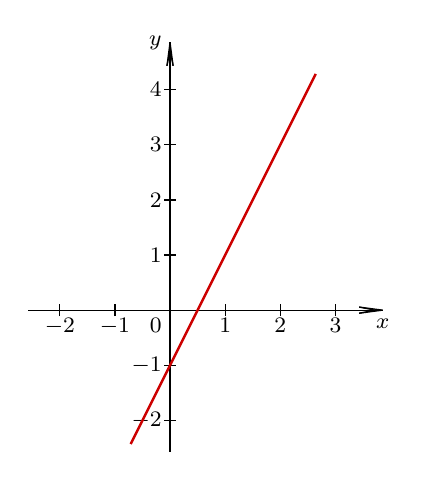
\begin{tikzpicture}
                        % \clip (0,0) rectangle (14.000000,10.000000);
                        {\footnotesize
                        
                        % Drawing 2D Cartesian system
                        \draw (3.000000,3.000000) node [anchor=north east] { $0$ };%
                        \draw [line width=0.016cm] (3.000000,2.925000) -- (3.000000,3.075000);%
                        \draw (3.700000,3.000000) node [anchor=north] { $1$ };%
                        \draw [line width=0.016cm] (3.700000,2.925000) -- (3.700000,3.075000);%
                        \draw (4.400000,3.000000) node [anchor=north] { $2$ };%
                        \draw [line width=0.016cm] (4.400000,2.925000) -- (4.400000,3.075000);%
                        \draw (5.100000,3.000000) node [anchor=north] { $3$ };%
                        \draw [line width=0.016cm] (5.100000,2.925000) -- (5.100000,3.075000);%
                        \draw (2.300000,3.000000) node [anchor=north] { $-1$ };%
                        \draw [line width=0.016cm] (2.300000,2.925000) -- (2.300000,3.075000);%
                        \draw (1.600000,3.000000) node [anchor=north] { $-2$ };%
                        \draw [line width=0.016cm] (1.600000,2.925000) -- (1.600000,3.075000);%
                        \draw (3.000000,3.700000) node [anchor=east] { $1$ };%
                        \draw [line width=0.016cm] (2.925000,3.700000) -- (3.075000,3.700000);%
                        \draw (3.000000,4.400000) node [anchor=east] { $2$ };%
                        \draw [line width=0.016cm] (2.925000,4.400000) -- (3.075000,4.400000);%
                        \draw (3.000000,5.100000) node [anchor=east] { $3$ };%
                        \draw [line width=0.016cm] (2.925000,5.100000) -- (3.075000,5.100000);%
                        \draw (3.000000,5.800000) node [anchor=east] { $4$ };%
                        \draw [line width=0.016cm] (2.925000,5.800000) -- (3.075000,5.800000);%
                        \draw (3.000000,2.300000) node [anchor=east] { $-1$ };%
                        \draw [line width=0.016cm] (2.925000,2.300000) -- (3.075000,2.300000);%
                        \draw (3.000000,1.600000) node [anchor=east] { $-2$ };%
                        \draw [line width=0.016cm] (2.925000,1.600000) -- (3.075000,1.600000);%
                        \draw (5.700000,3.000000) node [anchor=north] { $x$ };%
                        \draw (3.000000,6.400000) node [anchor=east] { $y$ };%
                        \draw [line width=0.016cm] (1.200000,3.000000) -- (5.700000,3.000000);%
                        \draw [line width=0.016cm] (5.402567,3.039158) -- (5.700000,3.000000);%
                        \draw [line width=0.016cm] (5.402567,3.039158) -- (5.600000,3.000000);%
                        \draw [line width=0.016cm] (5.402567,2.960842) -- (5.700000,3.000000);%
                        \draw [line width=0.016cm] (5.402567,2.960842) -- (5.600000,3.000000);%
                        \draw [line width=0.016cm] (3.000000,1.200000) -- (3.000000,6.400000);%
                        \draw [line width=0.016cm] (2.960842,6.102567) -- (3.000000,6.400000);%
                        \draw [line width=0.016cm] (2.960842,6.102567) -- (3.000000,6.300000);%
                        \draw [line width=0.016cm] (3.039158,6.102567) -- (3.000000,6.400000);%
                        \draw [line width=0.016cm] (3.039158,6.102567) -- (3.000000,6.300000);%
                        
                        % Changing color 204 0 0
                        \definecolor{r204g0b0}{rgb}{0.800000,0.000000,0.000000}%
                        \color{r204g0b0}% 
                        
                        % Drawing line l
                        \draw [line width=0.032cm] (2.500000,1.300000) -- (4.850000,6.000000);%
                        \color{black}
                        }
                        \end{tikzpicture}
                                                    
                \end{figure}

                \begin{figure}[H]
                    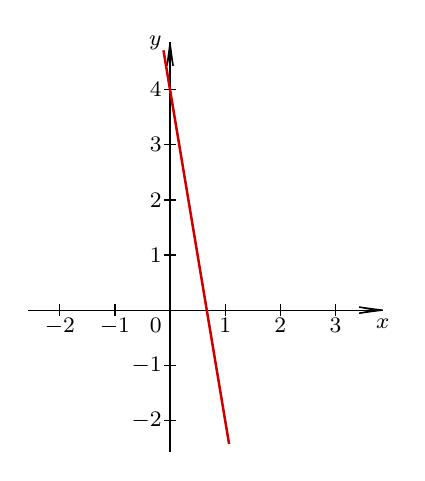
\begin{tikzpicture}
                        % \clip (0,0) rectangle (14.000000,10.000000);
                        {\footnotesize
                        
                        % Drawing 2D Cartesian system
                        \draw (3.000000,3.000000) node [anchor=north east] { $0$ };%
                        \draw [line width=0.016cm] (3.000000,2.925000) -- (3.000000,3.075000);%
                        \draw (3.700000,3.000000) node [anchor=north] { $1$ };%
                        \draw [line width=0.016cm] (3.700000,2.925000) -- (3.700000,3.075000);%
                        \draw (4.400000,3.000000) node [anchor=north] { $2$ };%
                        \draw [line width=0.016cm] (4.400000,2.925000) -- (4.400000,3.075000);%
                        \draw (5.100000,3.000000) node [anchor=north] { $3$ };%
                        \draw [line width=0.016cm] (5.100000,2.925000) -- (5.100000,3.075000);%
                        \draw (2.300000,3.000000) node [anchor=north] { $-1$ };%
                        \draw [line width=0.016cm] (2.300000,2.925000) -- (2.300000,3.075000);%
                        \draw (1.600000,3.000000) node [anchor=north] { $-2$ };%
                        \draw [line width=0.016cm] (1.600000,2.925000) -- (1.600000,3.075000);%
                        \draw (3.000000,3.700000) node [anchor=east] { $1$ };%
                        \draw [line width=0.016cm] (2.925000,3.700000) -- (3.075000,3.700000);%
                        \draw (3.000000,4.400000) node [anchor=east] { $2$ };%
                        \draw [line width=0.016cm] (2.925000,4.400000) -- (3.075000,4.400000);%
                        \draw (3.000000,5.100000) node [anchor=east] { $3$ };%
                        \draw [line width=0.016cm] (2.925000,5.100000) -- (3.075000,5.100000);%
                        \draw (3.000000,5.800000) node [anchor=east] { $4$ };%
                        \draw [line width=0.016cm] (2.925000,5.800000) -- (3.075000,5.800000);%
                        \draw (3.000000,2.300000) node [anchor=east] { $-1$ };%
                        \draw [line width=0.016cm] (2.925000,2.300000) -- (3.075000,2.300000);%
                        \draw (3.000000,1.600000) node [anchor=east] { $-2$ };%
                        \draw [line width=0.016cm] (2.925000,1.600000) -- (3.075000,1.600000);%
                        \draw (5.700000,3.000000) node [anchor=north] { $x$ };%
                        \draw (3.000000,6.400000) node [anchor=east] { $y$ };%
                        \draw [line width=0.016cm] (1.200000,3.000000) -- (5.700000,3.000000);%
                        \draw [line width=0.016cm] (5.402567,3.039158) -- (5.700000,3.000000);%
                        \draw [line width=0.016cm] (5.402567,3.039158) -- (5.600000,3.000000);%
                        \draw [line width=0.016cm] (5.402567,2.960842) -- (5.700000,3.000000);%
                        \draw [line width=0.016cm] (5.402567,2.960842) -- (5.600000,3.000000);%
                        \draw [line width=0.016cm] (3.000000,1.200000) -- (3.000000,6.400000);%
                        \draw [line width=0.016cm] (2.960842,6.102567) -- (3.000000,6.400000);%
                        \draw [line width=0.016cm] (2.960842,6.102567) -- (3.000000,6.300000);%
                        \draw [line width=0.016cm] (3.039158,6.102567) -- (3.000000,6.400000);%
                        \draw [line width=0.016cm] (3.039158,6.102567) -- (3.000000,6.300000);%
                        
                        % Changing color 204 0 0
                        \definecolor{r204g0b0}{rgb}{0.800000,0.000000,0.000000}%
                        \color{r204g0b0}% 
                        
                        % Drawing line l
                        \draw [line width=0.032cm] (3.750000,1.300000) -- (2.916667,6.300000);%
                        \color{black}
                        }
                        \end{tikzpicture}
                        
                \end{figure}

                \begin{figure}[H]
                    \begin{tikzpicture}
                        % \clip (0,0) rectangle (14.000000,10.000000);
                        {\footnotesize
                        
                        % Drawing 2D Cartesian system
                        \draw (3.000000,3.000000) node [anchor=north east] { $0$ };%
                        \draw [line width=0.016cm] (3.000000,2.925000) -- (3.000000,3.075000);%
                        \draw (3.700000,3.000000) node [anchor=north] { $1$ };%
                        \draw [line width=0.016cm] (3.700000,2.925000) -- (3.700000,3.075000);%
                        \draw (4.400000,3.000000) node [anchor=north] { $2$ };%
                        \draw [line width=0.016cm] (4.400000,2.925000) -- (4.400000,3.075000);%
                        \draw (5.100000,3.000000) node [anchor=north] { $3$ };%
                        \draw [line width=0.016cm] (5.100000,2.925000) -- (5.100000,3.075000);%
                        \draw (2.300000,3.000000) node [anchor=north] { $-1$ };%
                        \draw [line width=0.016cm] (2.300000,2.925000) -- (2.300000,3.075000);%
                        \draw (1.600000,3.000000) node [anchor=north] { $-2$ };%
                        \draw [line width=0.016cm] (1.600000,2.925000) -- (1.600000,3.075000);%
                        \draw (3.000000,3.700000) node [anchor=east] { $1$ };%
                        \draw [line width=0.016cm] (2.925000,3.700000) -- (3.075000,3.700000);%
                        \draw (3.000000,4.400000) node [anchor=east] { $2$ };%
                        \draw [line width=0.016cm] (2.925000,4.400000) -- (3.075000,4.400000);%
                        \draw (3.000000,5.100000) node [anchor=east] { $3$ };%
                        \draw [line width=0.016cm] (2.925000,5.100000) -- (3.075000,5.100000);%
                        \draw (3.000000,5.800000) node [anchor=east] { $4$ };%
                        \draw [line width=0.016cm] (2.925000,5.800000) -- (3.075000,5.800000);%
                        \draw (3.000000,2.300000) node [anchor=east] { $-1$ };%
                        \draw [line width=0.016cm] (2.925000,2.300000) -- (3.075000,2.300000);%
                        \draw (3.000000,1.600000) node [anchor=east] { $-2$ };%
                        \draw [line width=0.016cm] (2.925000,1.600000) -- (3.075000,1.600000);%
                        \draw (5.700000,3.000000) node [anchor=north] { $x$ };%
                        \draw (3.000000,6.400000) node [anchor=east] { $y$ };%
                        \draw [line width=0.016cm] (1.200000,3.000000) -- (5.700000,3.000000);%
                        \draw [line width=0.016cm] (5.402567,3.039158) -- (5.700000,3.000000);%
                        \draw [line width=0.016cm] (5.402567,3.039158) -- (5.600000,3.000000);%
                        \draw [line width=0.016cm] (5.402567,2.960842) -- (5.700000,3.000000);%
                        \draw [line width=0.016cm] (5.402567,2.960842) -- (5.600000,3.000000);%
                        \draw [line width=0.016cm] (3.000000,1.200000) -- (3.000000,6.400000);%
                        \draw [line width=0.016cm] (2.960842,6.102567) -- (3.000000,6.400000);%
                        \draw [line width=0.016cm] (2.960842,6.102567) -- (3.000000,6.300000);%
                        \draw [line width=0.016cm] (3.039158,6.102567) -- (3.000000,6.400000);%
                        \draw [line width=0.016cm] (3.039158,6.102567) -- (3.000000,6.300000);%
                        
                        % Changing color 204 0 0
                        \definecolor{r204g0b0}{rgb}{0.800000,0.000000,0.000000}%
                        \color{r204g0b0}% 
                        
                        % Drawing line l
                        \draw [line width=0.032cm] (4.900000,6.300000) -- (1.300000,2.700000);%
                        \color{black}
                        }
                        \end{tikzpicture}
                        
                \end{figure}



    


                \begin{figure}[H]
                    \begin{tikzpicture}
                        % \clip (0,0) rectangle (14.000000,10.000000);
                        {\footnotesize
                        
                        % Drawing 2D Cartesian system
                        \draw (3.000000,3.000000) node [anchor=north east] { $0$ };%
                        \draw [line width=0.016cm] (3.000000,2.925000) -- (3.000000,3.075000);%
                        \draw (3.700000,3.000000) node [anchor=north] { $1$ };%
                        \draw [line width=0.016cm] (3.700000,2.925000) -- (3.700000,3.075000);%
                        \draw (4.400000,3.000000) node [anchor=north] { $2$ };%
                        \draw [line width=0.016cm] (4.400000,2.925000) -- (4.400000,3.075000);%
                        \draw (5.100000,3.000000) node [anchor=north] { $3$ };%
                        \draw [line width=0.016cm] (5.100000,2.925000) -- (5.100000,3.075000);%
                        \draw (2.300000,3.000000) node [anchor=north] { $-1$ };%
                        \draw [line width=0.016cm] (2.300000,2.925000) -- (2.300000,3.075000);%
                        \draw (1.600000,3.000000) node [anchor=north] { $-2$ };%
                        \draw [line width=0.016cm] (1.600000,2.925000) -- (1.600000,3.075000);%
                        \draw (3.000000,3.700000) node [anchor=east] { $1$ };%
                        \draw [line width=0.016cm] (2.925000,3.700000) -- (3.075000,3.700000);%
                        \draw (3.000000,4.400000) node [anchor=east] { $2$ };%
                        \draw [line width=0.016cm] (2.925000,4.400000) -- (3.075000,4.400000);%
                        \draw (3.000000,5.100000) node [anchor=east] { $3$ };%
                        \draw [line width=0.016cm] (2.925000,5.100000) -- (3.075000,5.100000);%
                        \draw (3.000000,5.800000) node [anchor=east] { $4$ };%
                        \draw [line width=0.016cm] (2.925000,5.800000) -- (3.075000,5.800000);%
                        \draw (3.000000,2.300000) node [anchor=east] { $-1$ };%
                        \draw [line width=0.016cm] (2.925000,2.300000) -- (3.075000,2.300000);%
                        \draw (3.000000,1.600000) node [anchor=east] { $-2$ };%
                        \draw [line width=0.016cm] (2.925000,1.600000) -- (3.075000,1.600000);%
                        \draw (5.700000,3.000000) node [anchor=north] { $x$ };%
                        \draw (3.000000,6.400000) node [anchor=east] { $y$ };%
                        \draw [line width=0.016cm] (1.200000,3.000000) -- (5.700000,3.000000);%
                        \draw [line width=0.016cm] (5.402567,3.039158) -- (5.700000,3.000000);%
                        \draw [line width=0.016cm] (5.402567,3.039158) -- (5.600000,3.000000);%
                        \draw [line width=0.016cm] (5.402567,2.960842) -- (5.700000,3.000000);%
                        \draw [line width=0.016cm] (5.402567,2.960842) -- (5.600000,3.000000);%
                        \draw [line width=0.016cm] (3.000000,1.200000) -- (3.000000,6.400000);%
                        \draw [line width=0.016cm] (2.960842,6.102567) -- (3.000000,6.400000);%
                        \draw [line width=0.016cm] (2.960842,6.102567) -- (3.000000,6.300000);%
                        \draw [line width=0.016cm] (3.039158,6.102567) -- (3.000000,6.400000);%
                        \draw [line width=0.016cm] (3.039158,6.102567) -- (3.000000,6.300000);%
                        
                        % Changing color 204 0 0
                        \definecolor{r204g0b0}{rgb}{0.800000,0.000000,0.000000}%
                        \color{r204g0b0}% 
                        
                        % Drawing line l
                        \draw [line width=0.032cm] (1.300000,3.700000) -- (5.600000,3.700000);%
                        \color{black}
                        }
                        \end{tikzpicture}
                                                         
                \end{figure}


                \begin{figure}[H]
                    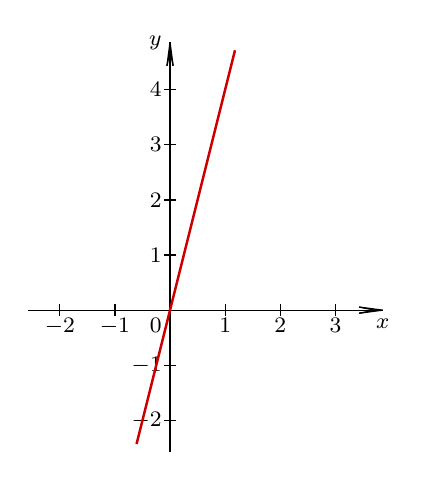
\begin{tikzpicture}
                        % \clip (0,0) rectangle (14.000000,10.000000);
                        {\footnotesize
                        
                        % Drawing 2D Cartesian system
                        \draw (3.000000,3.000000) node [anchor=north east] { $0$ };%
                        \draw [line width=0.016cm] (3.000000,2.925000) -- (3.000000,3.075000);%
                        \draw (3.700000,3.000000) node [anchor=north] { $1$ };%
                        \draw [line width=0.016cm] (3.700000,2.925000) -- (3.700000,3.075000);%
                        \draw (4.400000,3.000000) node [anchor=north] { $2$ };%
                        \draw [line width=0.016cm] (4.400000,2.925000) -- (4.400000,3.075000);%
                        \draw (5.100000,3.000000) node [anchor=north] { $3$ };%
                        \draw [line width=0.016cm] (5.100000,2.925000) -- (5.100000,3.075000);%
                        \draw (2.300000,3.000000) node [anchor=north] { $-1$ };%
                        \draw [line width=0.016cm] (2.300000,2.925000) -- (2.300000,3.075000);%
                        \draw (1.600000,3.000000) node [anchor=north] { $-2$ };%
                        \draw [line width=0.016cm] (1.600000,2.925000) -- (1.600000,3.075000);%
                        \draw (3.000000,3.700000) node [anchor=east] { $1$ };%
                        \draw [line width=0.016cm] (2.925000,3.700000) -- (3.075000,3.700000);%
                        \draw (3.000000,4.400000) node [anchor=east] { $2$ };%
                        \draw [line width=0.016cm] (2.925000,4.400000) -- (3.075000,4.400000);%
                        \draw (3.000000,5.100000) node [anchor=east] { $3$ };%
                        \draw [line width=0.016cm] (2.925000,5.100000) -- (3.075000,5.100000);%
                        \draw (3.000000,5.800000) node [anchor=east] { $4$ };%
                        \draw [line width=0.016cm] (2.925000,5.800000) -- (3.075000,5.800000);%
                        \draw (3.000000,2.300000) node [anchor=east] { $-1$ };%
                        \draw [line width=0.016cm] (2.925000,2.300000) -- (3.075000,2.300000);%
                        \draw (3.000000,1.600000) node [anchor=east] { $-2$ };%
                        \draw [line width=0.016cm] (2.925000,1.600000) -- (3.075000,1.600000);%
                        \draw (5.700000,3.000000) node [anchor=north] { $x$ };%
                        \draw (3.000000,6.400000) node [anchor=east] { $y$ };%
                        \draw [line width=0.016cm] (1.200000,3.000000) -- (5.700000,3.000000);%
                        \draw [line width=0.016cm] (5.402567,3.039158) -- (5.700000,3.000000);%
                        \draw [line width=0.016cm] (5.402567,3.039158) -- (5.600000,3.000000);%
                        \draw [line width=0.016cm] (5.402567,2.960842) -- (5.700000,3.000000);%
                        \draw [line width=0.016cm] (5.402567,2.960842) -- (5.600000,3.000000);%
                        \draw [line width=0.016cm] (3.000000,1.200000) -- (3.000000,6.400000);%
                        \draw [line width=0.016cm] (2.960842,6.102567) -- (3.000000,6.400000);%
                        \draw [line width=0.016cm] (2.960842,6.102567) -- (3.000000,6.300000);%
                        \draw [line width=0.016cm] (3.039158,6.102567) -- (3.000000,6.400000);%
                        \draw [line width=0.016cm] (3.039158,6.102567) -- (3.000000,6.300000);%
                        
                        % Changing color 204 0 0
                        \definecolor{r204g0b0}{rgb}{0.800000,0.000000,0.000000}%
                        \color{r204g0b0}% 
                        
                        % Drawing line l
                        \draw [line width=0.032cm] (2.575000,1.300000) -- (3.825000,6.300000);%
                        \color{black}
                        }
                        \end{tikzpicture}
                        
                \end{figure}


                \begin{figure}[H]
                    \begin{tikzpicture}
                        % \clip (0,0) rectangle (14.000000,10.000000);
                        {\footnotesize
                        
                        % Drawing 2D Cartesian system
                        \draw (3.000000,3.000000) node [anchor=north east] { $0$ };%
                        \draw [line width=0.016cm] (3.000000,2.925000) -- (3.000000,3.075000);%
                        \draw (3.700000,3.000000) node [anchor=north] { $1$ };%
                        \draw [line width=0.016cm] (3.700000,2.925000) -- (3.700000,3.075000);%
                        \draw (4.400000,3.000000) node [anchor=north] { $2$ };%
                        \draw [line width=0.016cm] (4.400000,2.925000) -- (4.400000,3.075000);%
                        \draw (5.100000,3.000000) node [anchor=north] { $3$ };%
                        \draw [line width=0.016cm] (5.100000,2.925000) -- (5.100000,3.075000);%
                        \draw (2.300000,3.000000) node [anchor=north] { $-1$ };%
                        \draw [line width=0.016cm] (2.300000,2.925000) -- (2.300000,3.075000);%
                        \draw (1.600000,3.000000) node [anchor=north] { $-2$ };%
                        \draw [line width=0.016cm] (1.600000,2.925000) -- (1.600000,3.075000);%
                        \draw (3.000000,3.700000) node [anchor=east] { $1$ };%
                        \draw [line width=0.016cm] (2.925000,3.700000) -- (3.075000,3.700000);%
                        \draw (3.000000,4.400000) node [anchor=east] { $2$ };%
                        \draw [line width=0.016cm] (2.925000,4.400000) -- (3.075000,4.400000);%
                        \draw (3.000000,5.100000) node [anchor=east] { $3$ };%
                        \draw [line width=0.016cm] (2.925000,5.100000) -- (3.075000,5.100000);%
                        \draw (3.000000,5.800000) node [anchor=east] { $4$ };%
                        \draw [line width=0.016cm] (2.925000,5.800000) -- (3.075000,5.800000);%
                        \draw (3.000000,2.300000) node [anchor=east] { $-1$ };%
                        \draw [line width=0.016cm] (2.925000,2.300000) -- (3.075000,2.300000);%
                        \draw (3.000000,1.600000) node [anchor=east] { $-2$ };%
                        \draw [line width=0.016cm] (2.925000,1.600000) -- (3.075000,1.600000);%
                        \draw (5.700000,3.000000) node [anchor=north] { $x$ };%
                        \draw (3.000000,6.400000) node [anchor=east] { $y$ };%
                        \draw [line width=0.016cm] (1.200000,3.000000) -- (5.700000,3.000000);%
                        \draw [line width=0.016cm] (5.402567,3.039158) -- (5.700000,3.000000);%
                        \draw [line width=0.016cm] (5.402567,3.039158) -- (5.600000,3.000000);%
                        \draw [line width=0.016cm] (5.402567,2.960842) -- (5.700000,3.000000);%
                        \draw [line width=0.016cm] (5.402567,2.960842) -- (5.600000,3.000000);%
                        \draw [line width=0.016cm] (3.000000,1.200000) -- (3.000000,6.400000);%
                        \draw [line width=0.016cm] (2.960842,6.102567) -- (3.000000,6.400000);%
                        \draw [line width=0.016cm] (2.960842,6.102567) -- (3.000000,6.300000);%
                        \draw [line width=0.016cm] (3.039158,6.102567) -- (3.000000,6.400000);%
                        \draw [line width=0.016cm] (3.039158,6.102567) -- (3.000000,6.300000);%
                        
                        % Changing color 204 0 0
                        \definecolor{r204g0b0}{rgb}{0.800000,0.000000,0.000000}%
                        \color{r204g0b0}% 
                        
                        % Drawing line l
                        \draw [line width=0.032cm] (2.700000,1.300000) -- (5.600000,4.200000);%
                        \color{black}
                        }
                        \end{tikzpicture}
                        
                \end{figure}



                \begin{figure}[H]
                    \begin{tikzpicture}
                        % \clip (0,0) rectangle (14.000000,10.000000);
                        {\footnotesize
                        
                        % Drawing 2D Cartesian system
                        \draw (3.000000,3.000000) node [anchor=north east] { $0$ };%
                        \draw [line width=0.016cm] (3.000000,2.925000) -- (3.000000,3.075000);%
                        \draw (3.700000,3.000000) node [anchor=north] { $1$ };%
                        \draw [line width=0.016cm] (3.700000,2.925000) -- (3.700000,3.075000);%
                        \draw (4.400000,3.000000) node [anchor=north] { $2$ };%
                        \draw [line width=0.016cm] (4.400000,2.925000) -- (4.400000,3.075000);%
                        \draw (5.100000,3.000000) node [anchor=north] { $3$ };%
                        \draw [line width=0.016cm] (5.100000,2.925000) -- (5.100000,3.075000);%
                        \draw (2.300000,3.000000) node [anchor=north] { $-1$ };%
                        \draw [line width=0.016cm] (2.300000,2.925000) -- (2.300000,3.075000);%
                        \draw (1.600000,3.000000) node [anchor=north] { $-2$ };%
                        \draw [line width=0.016cm] (1.600000,2.925000) -- (1.600000,3.075000);%
                        \draw (3.000000,3.700000) node [anchor=east] { $1$ };%
                        \draw [line width=0.016cm] (2.925000,3.700000) -- (3.075000,3.700000);%
                        \draw (3.000000,4.400000) node [anchor=east] { $2$ };%
                        \draw [line width=0.016cm] (2.925000,4.400000) -- (3.075000,4.400000);%
                        \draw (3.000000,5.100000) node [anchor=east] { $3$ };%
                        \draw [line width=0.016cm] (2.925000,5.100000) -- (3.075000,5.100000);%
                        \draw (3.000000,5.800000) node [anchor=east] { $4$ };%
                        \draw [line width=0.016cm] (2.925000,5.800000) -- (3.075000,5.800000);%
                        \draw (3.000000,2.300000) node [anchor=east] { $-1$ };%
                        \draw [line width=0.016cm] (2.925000,2.300000) -- (3.075000,2.300000);%
                        \draw (3.000000,1.600000) node [anchor=east] { $-2$ };%
                        \draw [line width=0.016cm] (2.925000,1.600000) -- (3.075000,1.600000);%
                        \draw (5.700000,3.000000) node [anchor=north] { $x$ };%
                        \draw (3.000000,6.400000) node [anchor=east] { $y$ };%
                        \draw [line width=0.016cm] (1.200000,3.000000) -- (5.700000,3.000000);%
                        \draw [line width=0.016cm] (5.402567,3.039158) -- (5.700000,3.000000);%
                        \draw [line width=0.016cm] (5.402567,3.039158) -- (5.600000,3.000000);%
                        \draw [line width=0.016cm] (5.402567,2.960842) -- (5.700000,3.000000);%
                        \draw [line width=0.016cm] (5.402567,2.960842) -- (5.600000,3.000000);%
                        \draw [line width=0.016cm] (3.000000,1.200000) -- (3.000000,6.400000);%
                        \draw [line width=0.016cm] (2.960842,6.102567) -- (3.000000,6.400000);%
                        \draw [line width=0.016cm] (2.960842,6.102567) -- (3.000000,6.300000);%
                        \draw [line width=0.016cm] (3.039158,6.102567) -- (3.000000,6.400000);%
                        \draw [line width=0.016cm] (3.039158,6.102567) -- (3.000000,6.300000);%
                        
                        % Changing color 204 0 0
                        \definecolor{r204g0b0}{rgb}{0.800000,0.000000,0.000000}%
                        \color{r204g0b0}% 
                        
                        % Drawing line l
                        \draw [line width=0.032cm] (1.300000,3.550000) -- (5.600000,5.700000);%
                        \color{black}
                        }
                        \end{tikzpicture}
                                              
                \end{figure}


                \begin{figure}[H]
                    \begin{tikzpicture}
                        % \clip (0,0) rectangle (14.000000,10.000000);
                        {\footnotesize
                        
                        % Drawing 2D Cartesian system
                        \draw (3.000000,3.000000) node [anchor=north east] { $0$ };%
                        \draw [line width=0.016cm] (3.000000,2.925000) -- (3.000000,3.075000);%
                        \draw (3.700000,3.000000) node [anchor=north] { $1$ };%
                        \draw [line width=0.016cm] (3.700000,2.925000) -- (3.700000,3.075000);%
                        \draw (4.400000,3.000000) node [anchor=north] { $2$ };%
                        \draw [line width=0.016cm] (4.400000,2.925000) -- (4.400000,3.075000);%
                        \draw (5.100000,3.000000) node [anchor=north] { $3$ };%
                        \draw [line width=0.016cm] (5.100000,2.925000) -- (5.100000,3.075000);%
                        \draw (2.300000,3.000000) node [anchor=north] { $-1$ };%
                        \draw [line width=0.016cm] (2.300000,2.925000) -- (2.300000,3.075000);%
                        \draw (1.600000,3.000000) node [anchor=north] { $-2$ };%
                        \draw [line width=0.016cm] (1.600000,2.925000) -- (1.600000,3.075000);%
                        \draw (3.000000,3.700000) node [anchor=east] { $1$ };%
                        \draw [line width=0.016cm] (2.925000,3.700000) -- (3.075000,3.700000);%
                        \draw (3.000000,4.400000) node [anchor=east] { $2$ };%
                        \draw [line width=0.016cm] (2.925000,4.400000) -- (3.075000,4.400000);%
                        \draw (3.000000,5.100000) node [anchor=east] { $3$ };%
                        \draw [line width=0.016cm] (2.925000,5.100000) -- (3.075000,5.100000);%
                        \draw (3.000000,5.800000) node [anchor=east] { $4$ };%
                        \draw [line width=0.016cm] (2.925000,5.800000) -- (3.075000,5.800000);%
                        \draw (3.000000,2.300000) node [anchor=east] { $-1$ };%
                        \draw [line width=0.016cm] (2.925000,2.300000) -- (3.075000,2.300000);%
                        \draw (3.000000,1.600000) node [anchor=east] { $-2$ };%
                        \draw [line width=0.016cm] (2.925000,1.600000) -- (3.075000,1.600000);%
                        \draw (5.700000,3.000000) node [anchor=north] { $x$ };%
                        \draw (3.000000,6.400000) node [anchor=east] { $y$ };%
                        \draw [line width=0.016cm] (1.200000,3.000000) -- (5.700000,3.000000);%
                        \draw [line width=0.016cm] (5.402567,3.039158) -- (5.700000,3.000000);%
                        \draw [line width=0.016cm] (5.402567,3.039158) -- (5.600000,3.000000);%
                        \draw [line width=0.016cm] (5.402567,2.960842) -- (5.700000,3.000000);%
                        \draw [line width=0.016cm] (5.402567,2.960842) -- (5.600000,3.000000);%
                        \draw [line width=0.016cm] (3.000000,1.200000) -- (3.000000,6.400000);%
                        \draw [line width=0.016cm] (2.960842,6.102567) -- (3.000000,6.400000);%
                        \draw [line width=0.016cm] (2.960842,6.102567) -- (3.000000,6.300000);%
                        \draw [line width=0.016cm] (3.039158,6.102567) -- (3.000000,6.400000);%
                        \draw [line width=0.016cm] (3.039158,6.102567) -- (3.000000,6.300000);%
                        
                        % Changing color 204 0 0
                        \definecolor{r204g0b0}{rgb}{0.800000,0.000000,0.000000}%
                        \color{r204g0b0}% 
                        
                        % Drawing line l
                        \draw [line width=0.032cm] (4.700000,1.300000) -- (1.300000,4.700000);%
                        \color{black}
                        }
                        \end{tikzpicture}
                        
                \end{figure}


                \begin{figure}[H]
                    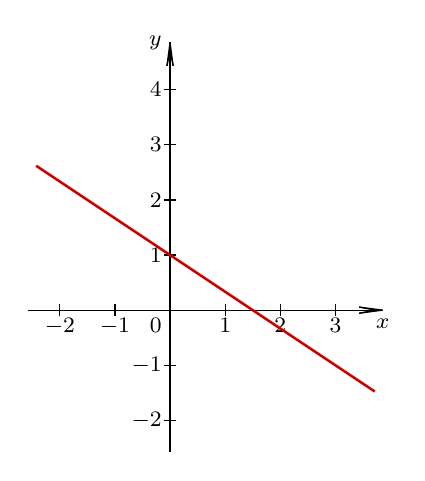
\begin{tikzpicture}
                        % \clip (0,0) rectangle (14.000000,10.000000);
                        {\footnotesize
                        
                        % Drawing 2D Cartesian system
                        \draw (3.000000,3.000000) node [anchor=north east] { $0$ };%
                        \draw [line width=0.016cm] (3.000000,2.925000) -- (3.000000,3.075000);%
                        \draw (3.700000,3.000000) node [anchor=north] { $1$ };%
                        \draw [line width=0.016cm] (3.700000,2.925000) -- (3.700000,3.075000);%
                        \draw (4.400000,3.000000) node [anchor=north] { $2$ };%
                        \draw [line width=0.016cm] (4.400000,2.925000) -- (4.400000,3.075000);%
                        \draw (5.100000,3.000000) node [anchor=north] { $3$ };%
                        \draw [line width=0.016cm] (5.100000,2.925000) -- (5.100000,3.075000);%
                        \draw (2.300000,3.000000) node [anchor=north] { $-1$ };%
                        \draw [line width=0.016cm] (2.300000,2.925000) -- (2.300000,3.075000);%
                        \draw (1.600000,3.000000) node [anchor=north] { $-2$ };%
                        \draw [line width=0.016cm] (1.600000,2.925000) -- (1.600000,3.075000);%
                        \draw (3.000000,3.700000) node [anchor=east] { $1$ };%
                        \draw [line width=0.016cm] (2.925000,3.700000) -- (3.075000,3.700000);%
                        \draw (3.000000,4.400000) node [anchor=east] { $2$ };%
                        \draw [line width=0.016cm] (2.925000,4.400000) -- (3.075000,4.400000);%
                        \draw (3.000000,5.100000) node [anchor=east] { $3$ };%
                        \draw [line width=0.016cm] (2.925000,5.100000) -- (3.075000,5.100000);%
                        \draw (3.000000,5.800000) node [anchor=east] { $4$ };%
                        \draw [line width=0.016cm] (2.925000,5.800000) -- (3.075000,5.800000);%
                        \draw (3.000000,2.300000) node [anchor=east] { $-1$ };%
                        \draw [line width=0.016cm] (2.925000,2.300000) -- (3.075000,2.300000);%
                        \draw (3.000000,1.600000) node [anchor=east] { $-2$ };%
                        \draw [line width=0.016cm] (2.925000,1.600000) -- (3.075000,1.600000);%
                        \draw (5.700000,3.000000) node [anchor=north] { $x$ };%
                        \draw (3.000000,6.400000) node [anchor=east] { $y$ };%
                        \draw [line width=0.016cm] (1.200000,3.000000) -- (5.700000,3.000000);%
                        \draw [line width=0.016cm] (5.402567,3.039158) -- (5.700000,3.000000);%
                        \draw [line width=0.016cm] (5.402567,3.039158) -- (5.600000,3.000000);%
                        \draw [line width=0.016cm] (5.402567,2.960842) -- (5.700000,3.000000);%
                        \draw [line width=0.016cm] (5.402567,2.960842) -- (5.600000,3.000000);%
                        \draw [line width=0.016cm] (3.000000,1.200000) -- (3.000000,6.400000);%
                        \draw [line width=0.016cm] (2.960842,6.102567) -- (3.000000,6.400000);%
                        \draw [line width=0.016cm] (2.960842,6.102567) -- (3.000000,6.300000);%
                        \draw [line width=0.016cm] (3.039158,6.102567) -- (3.000000,6.400000);%
                        \draw [line width=0.016cm] (3.039158,6.102567) -- (3.000000,6.300000);%
                        
                        % Changing color 204 0 0
                        \definecolor{r204g0b0}{rgb}{0.800000,0.000000,0.000000}%
                        \color{r204g0b0}% 
                        
                        % Drawing line l
                        \draw [line width=0.032cm] (1.300000,4.833220) -- (5.600000,1.966840);%
                        \color{black}
                        }
                        \end{tikzpicture}
                        
                \end{figure}


            \end{multicols}

        \end{naloga}

    



